\documentclass[a4paper,12pt]{article}
\usepackage{setspace}
\usepackage[margin=2.54cm]{geometry}
\usepackage{pdfpages}
\usepackage[utf8]{inputenc}
\usepackage[catalan]{babel}
\usepackage{graphicx,subcaption}
\usepackage{graphics}
\usepackage{lscape}
\usepackage{pdflscape}
\usepackage{float}
\usepackage{textcomp}
\usepackage{amsmath}
\usepackage{hyperref}
\usepackage{fancyvrb}
\usepackage{parskip}
\usepackage{changepage}
\usepackage{enumitem}
\usepackage{tcolorbox}
\usepackage[all]{hypcap}
\usepackage{xcolor}
\usepackage{listings}
\definecolor{green}{HTML}{228B22}
\definecolor{orange}{HTML}{FFA528}
\lstset{
    frame=tb, % draw a frame at the top and bottom of the code block
    tabsize=4, % tab space width
    showstringspaces=false, % don't mark spaces in strings
    numbers=left, % display line numbers on the left
    commentstyle=\color{green}, % comment color
    keywordstyle=\color{blue}, % keyword color
    stringstyle=\color{red}, % string color
    breaklines=true,
    numbers=left,
    xleftmargin=2em,
    framexleftmargin=1.5em,
    %postbreak=\mbox{\textcolor{red}{$\hookrightarrow$}\space},
}

\hypersetup{
    colorlinks,
    citecolor=black,
    filecolor=black,
    linkcolor=black,
    urlcolor=black
}
\title{
	\begin{center}
	\vspace{3cm}
	\includegraphics[width=11cm, height=3cm]{images/Logo-nou-eps.jpg}
	\end{center}
	\begin{center}
	\line(1,0){340}
	\end{center}		
	APRENENTATGE I RAONAMENT AUTOMÀTIC\\
	\vspace{2mm}
	\Large Pràctica 1: Agents amb lògica proposicional\\
	\line(1,0){340}
	\vspace{2.5cm}
	}

\author{Dand Marbà Sera - xxxxxxxxX \\   Marc Cervera Rosell - 47980320C \vspace{1cm}}


\date{25 d'abril  2022\vspace{0.5cm} \\Grau en Enginyeria Informàtica}
\onehalfspacing

\begin{document}
	\begin{titlepage}
		\maketitle
		\thispagestyle{empty}
	\end{titlepage}
	\cleardoublepage
	\newpage

\tableofcontents
\listoffigures
\thispagestyle{empty}

\newpage

\section{Disseny del programa}
\justify{Part del codi del cas pràctic, ha estat proporcionat per l'equip docent.
\\
\\
S'ha modificat l'estructura de manera que en el moment de tractar les posicions, es delegarà aquesta tasca a la classe \textit{Position}.
\\
\\
En segon lloc, s'ha afegit una classe anomenada \textit{PositionUtilities} que ofereix utilitats per poder obtenir la informació de les posicions del món. Concretament, permet saber quines son les posicions veïnes i si és una posició dins dels límits del món.
\\
\\
Referent al comportament del programa, l'agent comença generant la formula que li permet obtenir coneixement a mesura que es desplaça pel mapa. Per construir aquesta formula, es comença generant les clàusules on s'assumeix que pot haver sobres en qualsevol posició del món. Seguidament, és generen les clàusules que permeten descartar posicions i finalment, es generen les clàusules de consistència.
\\
\\
Posteriorment, el programa desplaça l'agent mentre a aquest li quedin moviments. En cada moviment l'agent es comunica amb l'entorn representat per la classe \textit{EnvelopeWorldEnv} mitjançant un missatge i si aquest es valida com a positiu, l'agent es desplaça i realitza les lectures del sensor comunicant-se novament amb l'entorn. \\
\\
Un cop rebudes les lectures, l'agent afegeix les evidències a la formula de tal manera que les variables del sensor es posaràn directament com una clàusula. En cas de no estar es posarà de forma negada.
\\
\\
Després d'afegir totes les evidències a la formula, l'agent processa les evidències per adquirir nou coneixement. Per poder fer una relitat aquest fet, l'agent utilitzarà el coneixement que ja te i les evidències i determinarà si pot o no descartar alguna de les posicions del món.
\\
\\
Per cada posició descartada, l'agent deduirà \neg $e_{x,y} ^ {t+1}$ i per tant, abans de seguir amb el següent moviment, actualitzarà el coneixement actual.
}

\pagenumbering{arabic}

\newpage

\section{Formula lògica proposicional utilitzada}
\subsection{Variables}


\begin{center}

    Variables = \{ $e_{x,y} ^ {t-1}$, $e_{x,y} ^ {t+1}$, $s1_{x,y} ^ {t}$, $s2_{x,y} ^ {t}$, $s3_{x,y} ^ {t}$ $|$ \forall x,y \ \in \ $[$ 1, n $]$ \ \times \ $[$ 1, n $]$ \}
    
\end{center}

\subsubsection{Significat de les variables}

\begin{itemize}
    \item $e_{x,y} ^ {t-1}$ : Aquesta variable especifica si en un instant de temps passat hi podía haver un sobre en la posició x,y.
    \item $e_{x,y} ^ {t+1}$ : Aquesta variable especifica el mateix que la variable anterior però en comptes de fer-ho en un temps passat, ho fa en un instant de temps futur.
    \item $s1_{x,y} ^ {t}$ : Aquesta variable, és una variable booleana que especifica si el sensor ha donat una lectura de valor 1 en un instant de temps en el present i en la posicó x,y.
    \item $s2_{x,y} ^ {t}$ : Aquesta variable, és una variable booleana que especifica si el sensor ha donat una lectura de valor 2 en un instant de temps en el present i en la posicó x,y.
    \item $s3_{x,y} ^ {t}$ : Aquesta variable, és una variable booleana que especifica si el sensor ha donat una lectura de valor 3 en un instant de temps en el present i en la posicó x,y.
\end{itemize}

\subsection{Clàusules}

\begin{enumerate}
    \item Conjunt de clàusules que asseguren la existència mínima d'un sobre.
    \begin{center}
        
        $($ $e_{1,1} ^ {t-1}$ \vee \ $e_{1,2} ^ {t-1}$ \ \vee \ ... \ \vee \ $e_{n,n} ^ {t-1}$ $)$ \ \wedge \ $($  $e_{1,1} ^ {t+1}$ \vee \ $e_{1,2} ^ {t+1}$ \ \vee \ ... \ \vee \ $e_{n,n} ^ {t+1}$ $)$
        
    \end{center}
    \item Clàusula que fa que el sistema sigui consitent
    \begin{center}
        
        \forall x,y \in $[$ 1,n $]$ \ \times \ $[$ 1,n $]$ $($ \neg $e_{x,y} ^ {t-1}$ \rightarrow \neg  $e_{x,y} ^ {t+1}$ $)$
        
    \end{center}
    
    \textbf{Nota: Per facilitar la codificació de les clausules, s'han definit dos predicats anomenats \textit{adjacentPositions} i \textit{diagonalPositions} que contenen les posicions adjacents i diagonals d'una posició (x,y) qualsevol. Som conscients que la definició de predicats no és compatible amb lògica proposicional, però hem cregut que la millor forma de facilitar la redacció d'aquest document era definir-los. Així mateix, el criteri seguit per introduïr a cada predicat les diferents posicions, és el que s'observa a la Figura~\ref{fig:posicions}.}
    
    \begin{figure}[H]
    \centering
	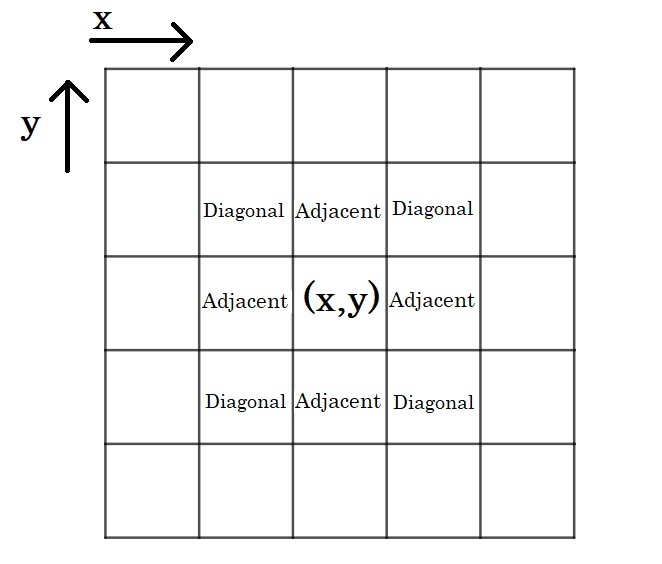
\includegraphics[scale = 0.7]{images/Position sets.jpg}
	\caption{Criteri de posicions}
	\label{fig:posicions}
\end{figure}
\justify{Per tant, dintre del conjunt \textit{AdjacentPositions} hi haurien les posicions: $(x+1, y)$, $(x-1, y)$, $(x, y+1)$, $(x, y-1)$. I dintre del conjunt \textit{DiagonalPositions} hi haurien les posicions:  $(x+1, y-1)$, $(x+1, y+1)$, $(x-1, y+1)$, $(x-1, y-1)$}

    \item Clàusules que donaràn com a valor de lectura del sensor un 1.
    \begin{center}
        
        \forall x,y \in \ $[$ 1,n $]$ \ \times \ $[$ 1,n $]$ $($ $s1_{x,y} ^ {t}$ \rightarrow \neg $e_{x',y'} ^ {t+1}$ $)$ \forall x',y' \in \textit{DiagonalPositions(x',y')} \land \forall (x',y') = (x, y)
        
    \end{center}
    
    \item Clàusules que donaràn com a valor de lectura del sensor un 2.
    \begin{center}
        
         \forall x,y \in \ $[$ 1,n $]$ \ \times \ $[$ 1,n $]$ $($ $s2_{x,y} ^ {t}$ \rightarrow \neg $e_{x',y'} ^ {t+1}$ $)$ \forall x',y' \in \textit{AdjacentPositions(x',y')} \land \forall (x',y') = (x, y)
        
    \end{center}
    
    \item Clàusules que donaràn com a valor de lectura del sensor un 3.
    \begin{center}
        
        \forall x,y \in \ $[$ 1,n $]$ \ \times \ $[$ 1,n $]$ $($ $s3_{x,y} ^ {t}$ \rightarrow \neg $e_{x',y'} ^ {t+1}$ $)$  \forall x',y' \in \textit{AdjacentPositions(x',y')} \land \textit{DiagonalPositions(x',y')}
        
    \end{center}
\end{enumerate}


\end{document}